\documentclass[11pt,UTF8]{ctexart}
\usepackage{titling}
\usepackage{enumerate}
\usepackage{amsmath}
\usepackage{amssymb}
\usepackage{amsfonts}
\usepackage{listings}
\usepackage{forest}
\usepackage{bm}
\usepackage{float}
\usepackage{graphicx}
\usepackage{multicol}
\usepackage[unicode=true,%本行非常重要 支持中文目录hyperref CJKbookmarks对二级目录没用
	colorlinks,
	linkcolor=black,
	anchorcolor=black,
	citecolor=black,
	CJKbookmarks=false]{hyperref}
\usepackage{xcolor}
\usepackage{geometry}
\geometry{top=20mm,bottom=20mm,left=20mm,right=20mm}
\pagestyle{plain}%删除页眉
\CTEXsetup[format={\Large\bfseries}]{section}

\setlength{\droptitle}{-50pt}%减少标题与页眉距离

\title{Project 2 技术报告}
\author{17341015 计一 陈鸿峥}
\date{}

\begin{document}
\maketitle
\vspace{-50pt}%减少标题与正文距离

\lstset{language=C++,escapechar=`}

\section{实验目的}
实现一个多项式计算器,可以进行简单的加减乘、求导等运算,并支持从文件读取和存储。

\section{实验环境}
采用 \verb'C++' 编写,在 \verb'Sublime Text 3' 上进行开发,并用 \verb'gcc 6.3.0' 编译,代码符合 \verb'C++11' 标准。

\section{实现思路}
多项式计算器的功能如下:
\begin{center}
\begin{forest}
for tree = {grow=south}
[多项式计算器
	[管理
		[添加多项式]
		[删除多项式]
		[显示所有多项式]]
	[计算
		[加减乘法]
		[求导]
		[赋值]
		[相等判断]]
	[存储
		[读取]
		[存储]]]
\end{forest}
\end{center}
\par 本多项式计算器主要分为管理、计算、存储三大模块。
\begin{enumerate}
	\item 管理模块\\
	包含添加多项式、删除多项式、显示所有多项式三个功能
	\item 计算模块\\
	包含加法、减法、乘法、求导、判断多项式相等、赋值共$6$个功能
	\item 存储模块\\
	包含读取数据和存储数据两个功能
\end{enumerate}


\section{设计细节}
\subsection{文件关系}
本多项式计算器包含三个源程序文件:
\begin{enumerate}
	\item \verb'polynomial_calculator.cpp' 为主文件,包含上述三个模块及具体的交互界面
	\item \verb'polynomial.hpp' 包含一个多项式类,实现单个多项式的存储及运算操作
	\item \verb'polynomials.hpp' 包含一个多项式仓库类,实现所有多项式的存储读取及多项运算
\end{enumerate}

\subsection{头文件}
\begin{enumerate}
	\item \verb'<string>',\verb'<vector>',\verb'<map>'为\verb'C++'标准库的容器,用于存储数据
	\item \verb'<iostream>',\verb'<fstream>'用于命令行及文件的输入输出
	\item \verb'<iomanip>'用于控制输出格式
	\item \verb'<regex>',\verb'<iterator>'为正则表达式和迭代器,用于字符串的分割
\end{enumerate}

\subsection{类结构设计}
\par 下图为\verb'Polynomial'类的实现,各个成员函数的含义均在命名中或是注释中表明,详情请见源码
\begin{figure}[H]
\centering
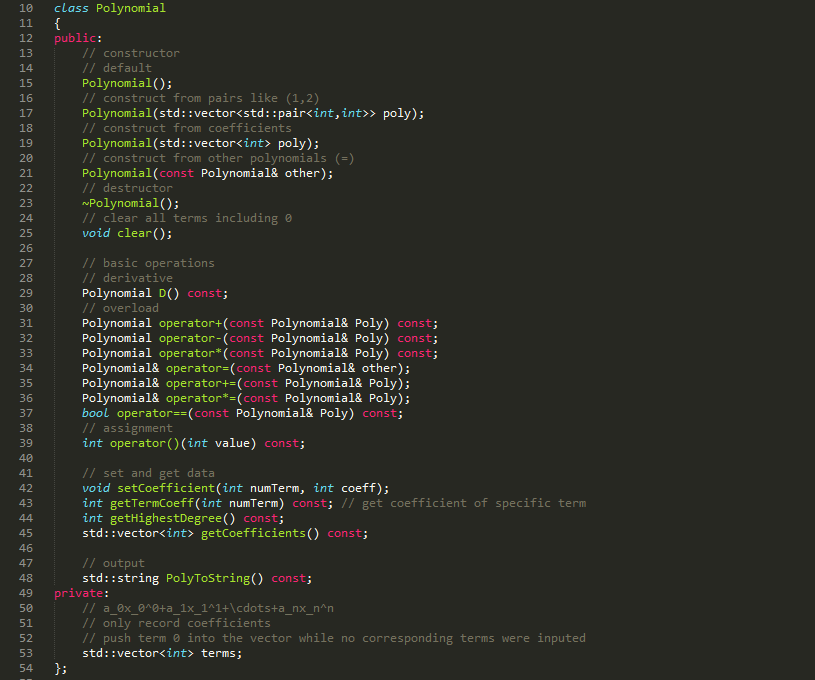
\includegraphics[width=\linewidth]{pic/class_polynomial.PNG}
\label{Fig:p1}
\end{figure}
\par 值得一提的特性:
\begin{enumerate}
	\item 类私有成员采用单个向量\verb'vector<int>'的形式存储,如$x^3+2x+1$则用$[1,0,2,1]$表示,没有项的系数用$0$补齐
	\item 提供了多种构造函数,支持多种构造方式
	\item 对几个运算符进行了重载,使得编写代码更加简便
	\item 由于存储某一多项式后\verb'terms'向量将不会清空,故经过运算后存在向量最高几维为$0$的情况,故特意引入\verb'getHighestDegree()'函数获取正确的最高次项
	\item \verb'PolyToString()'函数看似简单,但需要考虑的细节有很多
\end{enumerate}
\bigskip
\par 下图为\verb'Polynomials_'类的实现,各个成员函数的含义均在命名中或是注释中表明,详情请见源码
\begin{figure}[H]
\centering
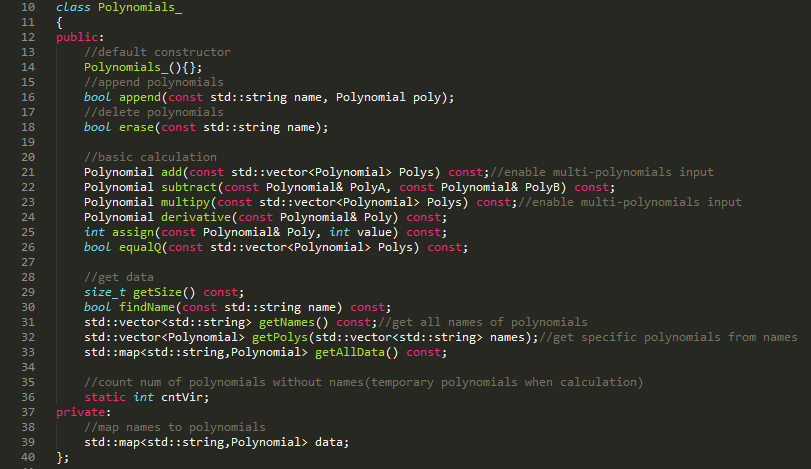
\includegraphics[width=\linewidth]{pic/class_polynomials.PNG}
\label{Fig:p2}
\end{figure}
\par 值得一提的特性:
\begin{enumerate}
	\item 类私有成员采用从名字到多项式的映射\verb'map<string,Polynomial>'存储
	\item 加法和乘法支持多个多项式同时运算,故函数输入是一个\verb'Polynomial'类型的\verb'vector'
	\item 减法支持一行内输入多个多项式,但只会对\textbf{前两个合法}的多项式进行操作
	\item 求导、等价判断同样支持一行内输入多个多项式,但只会对最前面一个合法多项式进行操作
	\item 引入了一个虚拟多项式(virtual polynomial),用于存储计算时直接输入的无名多项式,名字就定为\verb'Polynomials_::cntVir'的值,每次用完就删除;由于正常多项式的名字不允许出现数字(在\verb'validname_test'中保证),故名字为某一整数值不会与已有多项式冲突
\end{enumerate}

\subsection{主函数设计}
\par 主程序里的函数如下,具体实现请见代码
\begin{figure}[H]
\centering
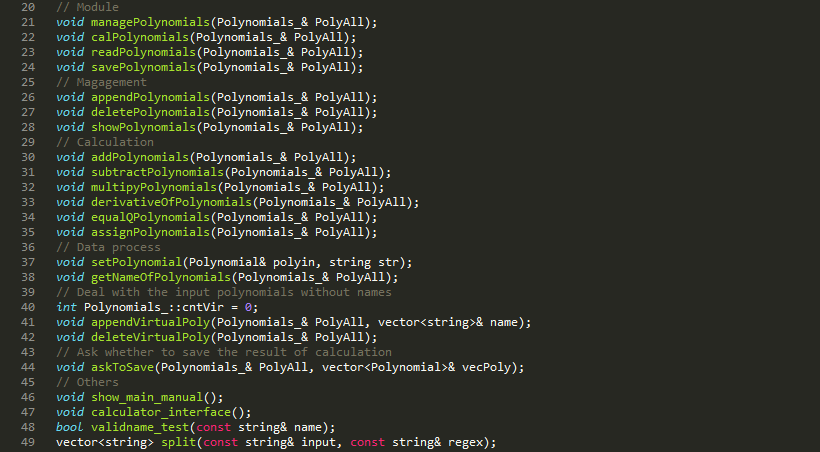
\includegraphics[width=\linewidth]{pic/main1.PNG}
\label{Fig:main1}
\end{figure}
\par 值得一提的细节:
\begin{enumerate}
	\item 每个模块均允许输入多个样例,并以\verb'END'结束输入
	\item 在每个计算之前均会给出说明及合法的例子,并且列出存储的多项式的名字
	\item $6$种计算操作均支持一行内多个输入,并且支持有名函数间运算、直接输入数对运算、或者交叉运算
	\item 结束本次计算都会进行询问是否需要保存计算结果
	\item 保存时考虑保存的编码是否在范围内、名字是否合法、名字是否冲突等
	\item \verb'appendPolynomial' 函数:实现多项式的读入到存储,数对\textbf{不一定}得降序输入
	\item \verb'setPolynomial' 函数:读入一个字符串(有序对)并对其进行分割(这里采用了正则表达式匹配),并存为\verb'pair'的形式,以便传入\verb'Polynomial'类的构造函数
	\item \verb'validname_test' 函数:判断名字是否合法,为避免冲突,多项式名只能为字母、短划线、下划线
	\item \verb'split' 函数(详情见下面代码):用\verb'C++'的正则表达式库编写,实现了与\verb'Python'的字符串分割函数\verb'split'类似的功能
\end{enumerate}
\begin{figure}[H]
\centering
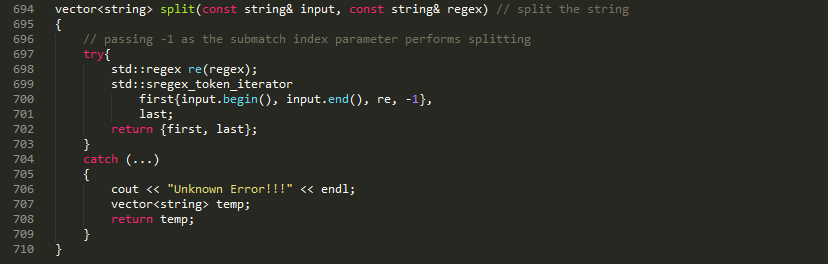
\includegraphics[width=\linewidth]{pic/split.PNG}
\label{Fig:split}
\end{figure}

\subsection{交互界面}
\begin{figure}[H]
\centering
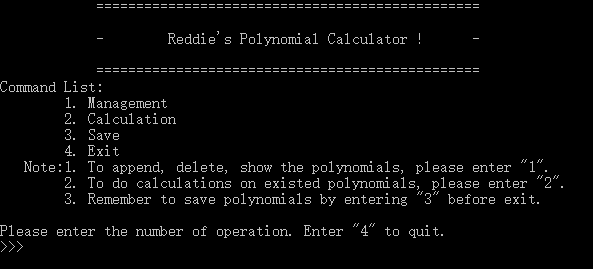
\includegraphics[width=\linewidth]{pic/interface.PNG}
\label{Fig:interface}
\end{figure}
\begin{itemize}
	\item 用\verb'<iomanip>'控制输出格式确保美观
	\item 用\verb'cin.clear()'和\verb'cin.sync()'清空缓存区,确保每次输入被程序读入后不会有残留,避免干扰下一次操作
	\item 当字符串长度为$0$或大于$1$时循环读入字符串,避免读入空行或者错误输入
	\item 多重输入判定,如在\verb'appendPolynomials'模块中(见下),会对输入名字的合法性、名字是否与已有多项式冲突等进行判定,确保输入准确合法
\end{itemize}
\begin{figure}[H]
\centering
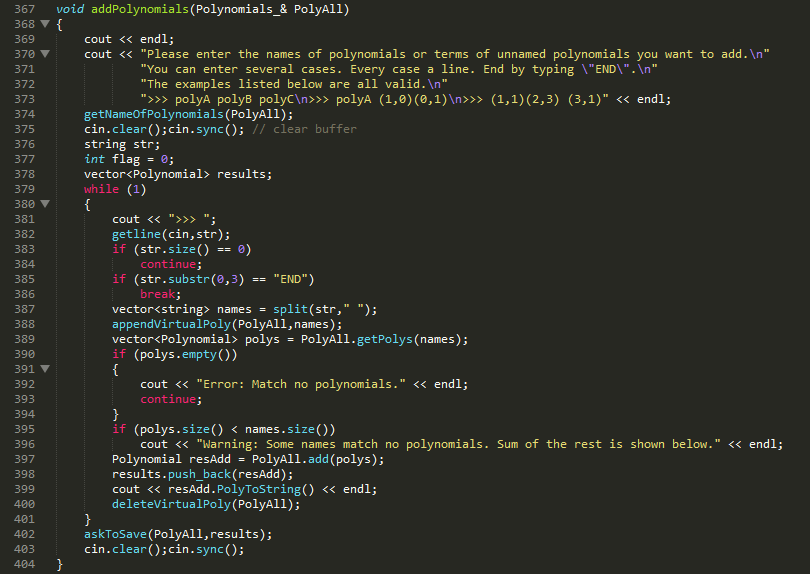
\includegraphics[width=\linewidth]{pic/add.PNG}
\label{Fig:add}
\end{figure}
\begin{figure}[H]
\centering
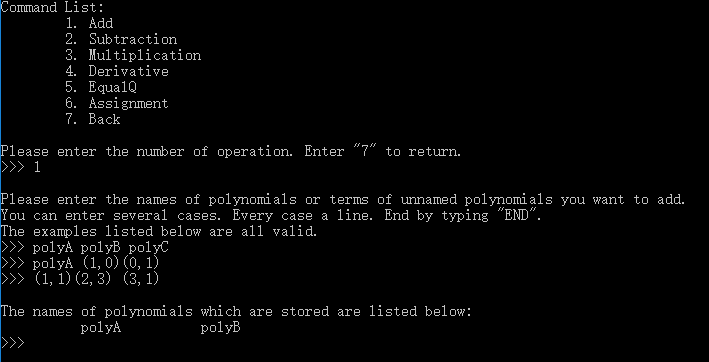
\includegraphics[width=\linewidth]{pic/add2.PNG}
\label{Fig:add2}
\end{figure}

\subsection{输入输出}
\begin{enumerate}
	\item 输出可在命令行中手动输入,或者从文件流中直接读入
	\item 输出同时有命令行的输出和文件流的输出(但要选择保存),输出格式同输入,即数对的列举,如$p=(1,2)(3,4)$
	\item 具体操作在交互界面均会提示,按照提示要求进行即可
\end{enumerate}


\section{程序测试及实验结果}
\par 实现了项目要求的所有功能,并且自行添加了multicases、multipolynomials等特性。
\par 写了$1000+$行代码考虑了各种极端情况,确保程序足够鲁棒。以下是调试时出现的一些问题及解决方案,以及用到的\verb'C++11'特性:
\begin{enumerate}
	\item \verb'split'函数在进行正则匹配时常常会导致程序崩溃:\\
		加上\verb'try,catch'特性捕获并避免发生异常
	\item 重载等号运算符后赋值老是会多出一项:\\
	在等号赋值前一定要将数据全部清空,包括第$0$项
	\item 赋值导致程序崩溃:\\
	赋值函数引用记得要返回\verb'*this'
	\item 必要的地方都加上const限定,防止误操作修改类的私有数据
	\item \verb'term.size()'是\verb'unsigned int'类型,对它$-1$会变为一个超大正数,故要先进行类型转换
	\item 使用\verb'auto'自动推断类型
	\item 使用\verb'for'的范围语句简化代码
	\item 使用\verb'rbegin'和\verb'rend'实现反向容器索引
\end{enumerate}


\section{心得体会}
\begin{enumerate}
	\item 第一次写项目写出千行代码,很开心!!!
	\item 调bug太难受了!!!
\end{enumerate}


\end{document}